\documentclass[uplatex,dvipdfmx]{jsarticle}
%参考文献
\usepackage[super]{cite}
\usepackage{url}
\renewcommand\citeform[1]{[#1]}

% 数式
\usepackage{amsthm,amsmath,amssymb,amsfonts}
\usepackage{physics}
\usepackage{bm}
\usepackage{mathtools}
\usepackage{siunitx}

% 画像
\usepackage[dvipdfmx]{graphicx}
\usepackage[hang,small,bf]{caption}
\usepackage[subrefformat=parens]{subcaption}
\captionsetup{compatibility=false}
\usepackage{hyperref}

% 図形
\usepackage{float}
\usepackage{tikz}
\usepackage{circuitikz}

% 自分用設定
\newcommand{\Frac}[2]{\dfrac{\,#1\,}{\,#2\,}}
\numberwithin{equation}{section}
\setcounter{tocdepth}{3}
\begin{document}
\title{\LaTeX の使い方} 
\author{うたおじ}
\date{}
\maketitle
uplatexを使って実験レポを書けるように、必要最低限くらいの知識をまとめようと思います。platexやlualatexを使いたいひとは、自分で調べてください。
\section{環境構築}
本節は「\href{https://qiita.com/rainbartown/items/d7718f12d71e688f3573}{VSCode で最高の LaTeX 環境を作る}」を参考にしてます(一部変更点あり)

URLは https://qiita.com/rainbartown/items/d7718f12d71e688f3573
\subsection{LaTeXのダウンロード}
\subsubsection{ダウンロード方法}
texliveを利用します。(MacユーザーはMacTeXを利用)1,2時間はかかります。スペックがクソゴミなPCだと7時間かかる例もあるそうです。パソコンを放置できるときにやりましょう。(ダウンロード途中で電源落ちたりすると悲惨なので注意)
\begin{itemize}
  \item Windowsユーザーの場合
  \begin{itemize}
    \item TeX Liveをダウンロードしましょう
    \item \href{https://tug.org/texlive/acquire-netinstall.html}{公式サイト}のinstall-tl-windows.exeをクリック
    \item 上記リンクが機能しない場合は https://tug.org/texlive/acquire-netinstall.html で検索してください
  \end{itemize}
  \item Macユーザーの場合
  \begin{itemize}
    \item brew install mactex-no-gui --cask で頑張れ(Macユーザーじゃないから俺は知らん)
  \end{itemize}
  \item linux(Ubuntu)ユーザーの場合
  \begin{itemize}
    \item sudo apt install texlive-full で頑張れ(linuxユーザーじゃないから俺は知らん)
  \end{itemize}
\end{itemize}
一部機能のみをダウンロードすることで時短はできますが、当然機能に制限がかかります。
\subsubsection{ちゃんとダウンロードできたか確認}
先に進む前に、ちゃんとダウンロードできたか確認しておきましょう。

スタートメニューを開き(winキーをクリック)、ターミナルを起動してください。できたら「latex -version」と打ち込みます。

次ページ図のように出力されれば、正常にインストールできています。『~として認識されていません』などと出力された場合は……インストールできてないのでやり直しです。
\begin{figure}[htbp]
  \centering
  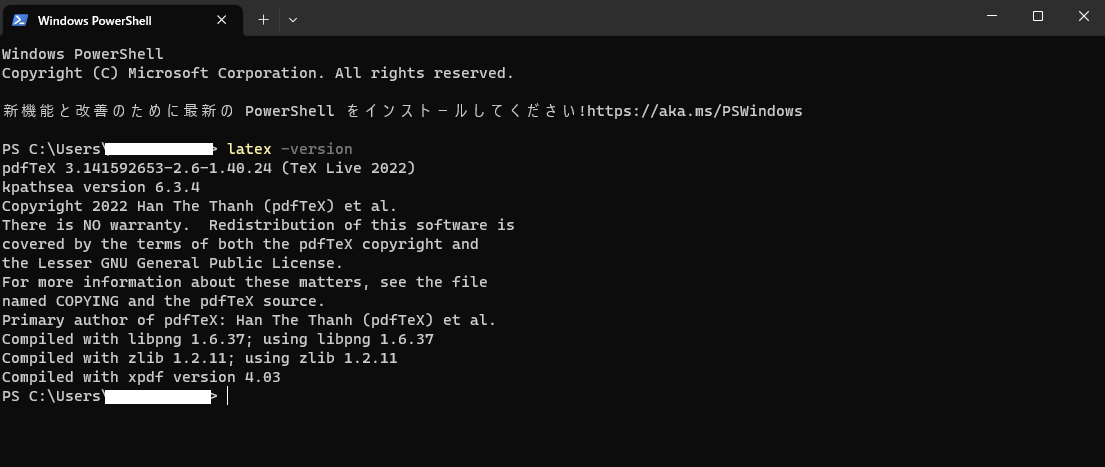
\includegraphics[width=0.7\linewidth]{powershell.png}
\end{figure}
\subsection*{VSCodeのダウンロード}
\LaTeX にデフォで存在するエディタは不便極まりないので、プログラマーに大人気のVisual Studio Code(以下VSCode)を使いましょう。Windowsにデフォのメモ帳でもかけるっちゃかけるけどそんなことやってるやつ見たことないです。

\href{https://code.visualstudio.com/download}{公式サイト}から、ダウンロードできます。

上記リンクが機能しない場合は https://code.visualstudio.com/download で検索
\subsection*{VSCodeの設定}
\subsubsection{拡張機能の追加}
まずは拡張機能を導入しましょう。導入するのは次の2つです。
\begin{itemize}
  \item Japanese Language Pack for Visual Studio Code
  \item LaTeX Workshop
\end{itemize}
私の環境ではすでに色々入れてるのでアイコンがちょっと多いですが、次の画像のようにすればインストールできます。LaTeX Workshop についても同様に、latexと検索してインストールしてください。
\subsubsection{settings.jsonの編集}
VSCodeの左下の歯車マークをクリックし、『設定』を開き、右上にある三点マークの2つ左にあるマークをクリックすると、settings.jsonがひらけます。
\subsection*{latexmkの設定}
\LaTeX のソースをpdf化する際、コマンドをいくつか入力しなければなりません。が、面倒ですよね。というわけで自動化しましょう。

\section{基本構造}
\section{文章の書き方}
ここでも簡易的には説明するものの、詳しくは自分で調べたり試行錯誤したりすることをおススメします。
ついでに参考になるサイト(参考にしたサイト)をまとめときます
\begin{itemize}
  \item \href{http://www.yamamo10.jp/yamamoto/comp/latex/make_doc/cover/index.php}{Yamamoto's Laboratory}
  \item \href{http://hooktail.org/computer/index.php?TeX}{物理のかぎしっぽ}
  \item \href{https://texwiki.texjp.org/}{TeX Wiki}
  \item その他、Quiitaなどのブログサイト
  \item \LaTeX を使ってる人に直接聞く(俺が暇な時であれば相談に乗ります)
\end{itemize}
また、次のようなことを調べたいときは以下のサイトがおススメです
\begin{itemize}
  \item \LaTeX の書き方のマナーを調べたいときは『\href{https://qiita.com/birdwatcher/items/5ec42b35d84d3ee2ffbb}{LaTeXにおける正しい論文の書き方}』
  \item 数式の表示にどんな種類があるのかは『\href{https://mathlandscape.com/latex-eq/#toc2}{LaTeX】数式環境まとめ【amsmath}』
\end{itemize}


\subsection*{小節・段落}
\subsection*{箇条書き}
\subsection*{title}
\section{数式の書き方}
\section{図表の書き方}
\section{応用}
\subsection{文書が長くなりすぎて実行に時間がかかりすぎる問題}
余裕で2桁ページに到達するような実験レポートを書いていると、pdf化に数十秒かかるようになってきます(PCのスペックによる?)これでは、今書いている内容が正しく表示されるか確認するだけで時間が過ぎ去っていくので、対策必須です。

あああ
\begin{itemize}
  \item[対策1] 編集する部分だけ取り出して、エラーを吐かなければメイン文書に統合
  \item[対策2] 分割して書けるパッケージ導入
\end{itemize}
対策1の方でも問題ないけれど、分割して書くシステムを作っておけば複数人での論文作成時にも応用できて便利です。

\end{document}